% Template for PLoS
% Version 2.0 July 2014
%
% To compile to pdf, run:
% latex plos.template
% bibtex plos.template
% latex plos.template
% latex plos.template
% dvipdf plos.template
%
% % % % % % % % % % % % % % % % % % % % % %
%
% -- IMPORTANT NOTE
%
% Be advised that this is merely a template 
% designed to facilitate accurate translation of manuscript content 
% into our production files. 
%
% This template contains extensive comments intended 
% to minimize problems and delays during our production 
% process. Please follow the template 
% whenever possible.
%
% % % % % % % % % % % % % % % % % % % % % % % 
%
% Once your paper is accepted for publication and enters production, 
% PLEASE REMOVE ALL TRACKED CHANGES in this file and leave only
% the final text of your manuscript.
%
% DO NOT ADD EXTRA PACKAGES TO THIS TEMPLATE unless absolutely necessary.
% Packages included in this template are intentionally
% limited and basic in order to reduce the possibility
% of issues during our production process.
%
% % % % % % % % % % % % % % % % % % % % % % %
%
% -- FIGURES AND TABLES
%
% DO NOT INCLUDE GRAPHICS IN YOUR MANUSCRIPT
% - Figures should be uploaded separately from your manuscript file. 
% - Figures generated using LaTeX should be extracted and removed from the PDF before submission. 
% - Figures containing multiple panels/subfigures must be combined into one image file before submission.
% See http://www.plosone.org/static/figureGuidelines for PLOS figure guidelines.
%
% Tables should be cell-based and may not contain:
% - tabs/spacing/line breaks within cells to alter layout
% - vertically-merged cells (no tabular environments within tabular environments, do not use \multirow)
% - colors, shading, or graphic objects
% See http://www.plosone.org/static/figureGuidelines#tables for table guidelines.
%
% For sideways tables, use the {rotating} package and use \begin{sidewaystable} instead of \begin{table} in the appropriate section. PLOS guidelines do not accomodate sideways figures.
%
% % % % % % % % % % % % % % % % % % % % % % % %
%
% -- EQUATIONS, MATH SYMBOLS, SUBSCRIPTS, AND SUPERSCRIPTS
%
% IMPORTANT
% Below are a few tips to help format your equations and other special characters according to our specifications. For more tips to help reduce the possibility of formatting errors during conversion, please see our LaTeX guidelines at http://www.plosone.org/static/latexGuidelines
%
% Please be sure to include all portions of an equation in the math environment, and for any superscripts or subscripts also include the base number/text. For example, use $mathrm{mm}^2$ instead of mm$^2$ (do not use \textsuperscript command).
%
% DO NOT USE the \rm command to render mathmode characters in roman font, instead use $\mathrm{}$
% For bolding characters in mathmode, please use $\mathbf{}$ 
%
% Please add line breaks to long equations when possible in order to fit our 2-column layout. 
%
% For inline equations, please do not include punctuation within the math environment unless this is part of the equation.
%
% For spaces within the math environment please use the \; or \: commands, even within \text{} (do not use smaller spacing as this does not convert well).
%
%
% % % % % % % % % % % % % % % % % % % % % % % %



\documentclass[10pt]{article}



% amsmath package, useful for mathematical formulas
\usepackage{amsmath}
% amssymb package, useful for mathematical symbols
\usepackage{amssymb}

% cite package, to clean up citations in the main text. Do not remove.
\usepackage{cite}

\usepackage{hyperref}

% line numbers
\usepackage{lineno}

% ligatures disabled
\usepackage{microtype}
\DisableLigatures[f]{encoding = *, family = * }

% rotating package for sideways tables
%\usepackage{rotating}

% If you wish to include algorithms, please use one of the packages below. Also, please see the algorithm section of our LaTeX guidelines (http://www.plosone.org/static/latexGuidelines) for important information about required formatting.
%\usepackage{algorithmic}
%\usepackage{algorithmicx}

% Use doublespacing - comment out for single spacing
%\usepackage{setspace} 
%\doublespacing


% Text layout
\topmargin 0.0cm
\oddsidemargin 0.5cm
\evensidemargin 0.5cm
\textwidth 16cm 
\textheight 21cm

% Bold the 'Figure #' in the caption and separate it with a period
% Captions will be left justified
\usepackage[labelfont=bf,labelsep=period,justification=raggedright]{caption}

% Use the PLoS provided BiBTeX style
\bibliographystyle{plos2009}

% Remove brackets from numbering in List of References
\makeatletter
\renewcommand{\@biblabel}[1]{\quad#1.}
\makeatother


% Leave date blank
\date{}

\pagestyle{myheadings}

%% Include all macros below. Please limit the use of macros.

%% END MACROS SECTION


\begin{document}


% Title must be 150 characters or less
\begin{flushleft}
{\Large
\textbf{3D-Printed Oxygen Control Devices}
}
% Insert Author names, affiliations and corresponding author email.
\\
Martin D. Brennan$^{1}$, 
Megan L. Rexius-Hall$^{1}$, 
David T. Eddington$^{1,\ast}$
\\
\bf{1} Dept of Bioengineering, University of Illinois at Chicago, Chicago, Illinois, USA
\\
%\bf{2} Author2 Dept/Program/Center, Institution Name, City, State, Country
%\\
%\bf{3} Author3 Dept/Program/Center, Institution Name, City, State, Country
%\\
$\ast$ E-mail: Corresponding dte@uic.edu
\end{flushleft}

% Please keep the abstract between 250 and 300 words
\section*{Abstract}

Recently 3D printing has emerged as a method for directly printing complete microfluidic chips, 
although printing materials have been limited to non-oxygen permeable materials.
We demonstrate the addition of gas permeable PDMS (Polydimethylsiloxane) membranes to 3D printed microfluidic devices as a means to enable oxygen control cell culture studies.
%Two devices are presented and characterized.


% Please keep the Author Summary between 150 and 200 words
% Use first person. PLOS ONE authors please skip this step. 
% Author Summary not valid for PLOS ONE submissions.   
\section*{Author Summary}



\section*{Introduction}

3D printing of microfluidic devices enables rapid, one-step fabrication of complex designs infeasible to make with planar lithography and replica molding techniques.
In addition, planar lithography is time consuming, requires specialized equipment and facilities, and has a high failure rate.
It is not unusual for labs to make ten microfluidic devices to guarnantee one will work properly.
On the other hand, 3D CAD printing allows for unambiguous specifications and nearly eliminates time and effort spent on fabrication which is outsourced to a 3D printing company for around \$100/device \cite{Au2014,Chen2014}.
3D printing also allows integration of complex geometeries not possible with planar lithograpy, such as hose barbs and leur fittings.
Dissemination and distributed production is also vastly simplified due to easy shareing the design as a CAD file.
Due to these inherent advantages 3D printing has emerged as a method for directly printing complete microfluidic devices \cite{Au2014, Chen2014} (Poland guy?, UK guy?) 
Printing is currently limited in choice of materials when compared to MEMS style fabrication. 
As of yet there is no widely available methods or materials to facilitate direct printing of gas permeable materials.
Microfluidic cell culture devices are often made out of gas periable PDMS via soft photo lithography.
PDMS is a convient material for cell studies due to it's biocompatability, optical properties, and gas periability, faciliataing oxygen control of cell environments.
Oxygen control in cells studies is often overlooked by researchers, but important for mimicing conditions expericend by cells in vivo.

Oxygen control mulitwell inserts have been previously developed cast entirely from PDMS for 6 well culture plates. \cite{Oppegard2009, Oppegard2010}.
For a similar design to be scaled scaled (replicated) to a 24-well plate the fabriation becomes to tedious and error prone to be done by hand.
Moveing to 3D printing for the fabrication allowed futher features to be incoporated such as integrated distubtion channels and hose barbs, while elminating fabrication time and yeild.
Although avalible 3D pritable materials are non-gas-permiable, the addition of a PDMS membrane allows gas transfer. 
The previous 6-well PDMS device featured paralene coating to eliminate exchange of gas in th PDMS bulk. 
\bf{Motovation for oxygen control, what we have done previously in oxygen and sepcificly the 6-well plate and why we need to do this with a 3D printer. Also a bit on negative pressure Vs. positive pressure. - I don't have any data or any reason that I can prove for doing this. I was orginally afraid that the membranes would come off from the pressure.
Here we report on the development of 3D printed microfluidic devices for the control of oxygen in cell culture microenvironments.
We demonstrate a device that nests into a 24 well culture plate to control gas in each row of the plate independently of the incubators's condition.

% You may title this section "Methods" or "Models". 
% "Models" is not a valid title for PLoS ONE authors. However, PLoS ONE
% authors may use "Analysis" 
\section*{Materials and Methods}

%The 3-inch (75 mm) petri dish device contains a 500 $\mu$m wide channel following a serpentine path leaving 500 $\mu$m of spacing between channels and has integrated hose barbs directly printed onto the device.
%The 3D part is printed with the channels embedded in the bottom of the petri dish. 
%A 120 $\mu$m thick PDMS membrane is adhered across the channels by spin coating a thin layer of PDMS on the membrane and allowing it to cure in place.
%The device is designed so that a standard 3” petri dish lid may be used.
%This device allows cell culture in a large open well format compatible with assays requiring cell scraping.
%The membrane is easily peeled away allowing additional fixing/staining assays to be preformed and can also be replaced with a new membrane to reuse the device. 

The device was designed to integrate with a multiwell format, specifically an off-the-shelf 24 well plate. 
The 24 well plate insert is designed to control gas in 6 wells of a 24 well culture plate from one input, borrowing the working principle of previous work\cite{oppegard2010} and also incorporates integrated hose barbs to simplify device operation.
The pillars extend into each well leaving a $\sim$500 $\mu$m gap for media between the diffusion membrane and the culture surface at the bottom of the well.
Diffusion occurs rapidly across this gap allowing control of the dissolved gas environment around the cells. 
A distribution network stems from the central input that equalizes the flow along each path length by varying the channel width to the proximal, intermediate, and distal wells (Figure \ref{device-photos-figure}.

The device also features a ‘pipe within a pipe’ design so that gas flow enters and leaves the diffusion area in a uniform, and symmetrical flow pattern, which would not be possible with standard lithography and demonstrates the capabilities of 3D printing (Figure \ref{piller-well-render-figure}.
Again the membranes are adhered with a thin layer of PDMS on the membrane and allowed to cure in place.

The device was printed by Fineline Prototyping in Watershed XC using stereolithography.
CAD models were designed and printed with microfluidic delivery channels, and then completed by 
adhering a gas permeable membrane of PDMS to enable diffusion of gas to the culture area. 

\subsection*{Oxygen characterization}

Oxygen was measured with PtOEPK (Pt(II) Octaethylporphine ketone) planar sensors that were fixed to the bottom of a 24 well plate. 
The intensity of the sensor was measured and correlated to the concentration of oxygen with Stern-Volmer analysis (Figure \ref{piller-well-render-figure}.
Gas was perfused through the device with negative pressure to eliminate bubbles.
The inlet tubing was placed in a cone with with a flow that exceed the vacuum flow rate so that the vacuum was always pulling in the gas of interest and not the room air.
All gas tanks used in the oxygen characterization were 5\% CO2 in addition to the desired gas mix in anticipation of cell culture experiments as CO2 can alter the fluorescence of the PtOEPK.

\subsection*{Cell culture and hypoxia assay}

% Results and Discussion can be combined.
\section*{Results and Discussion}

%Oxygen was measured in the 3” petri dish device with a commercial fiber­optic probe (Figure 2).
%Oxygen control was demonstrated with gas flowing through the channel under the PDMS membrane.

The 24 well insert device was quantified with a platinum based (PtOEPK) planar oxygen sensor as shown in Figure \ref{oxygen-char-figure}.
Oxygen control was able to be controlled in each of the 6 wells equally from one gas input demonstrating the distribution network.
The device reaches steady state in 30 minutes and can then hold the oxygen level near 0\% indefinitely, while 100\% nitrogen is pumped through the device. 
\bf{reach different levels.}

% We only support three levels of headings, please do not create a heading level below \subsubsection.
\subsection*{Subsection 1}

\subsubsection*{SubSubsection 1.1}

\subsection*{Subsection 2}

%\section*{Discussion}

\section*{Conclusion}
3D printing microfluidic chips have been limited to non oxygen permeable materials.
We demonstrate oxygen control in 3D printed devices the addition of a gas permeable PDMS membrane. 
Oxygen control is demonstrated in a open well petri dish design and a 24 well plate.
3D printing allows complex designs, integrated tubing connectors, and is comparable in price to standard PDMS fabrication.
This technique represents a bridge to commercialization where robust devices can be more easily shared and disseminated.
While injection molding, hot embossing, or other industrial processes are cheaper when making hundreds to thousands of devices, it is not practical to make a injection mold when making tens to hundreds of devices.
In addition, PDMS fabrication would be too time consuming, expensive, and the failure rate would be unacceptable.
3D printing is a perfect solution to these device fabrication needs.


% Do NOT remove this, even if you are not including acknowledgments.

\section*{Acknowledgments}

This work funded by NSF 1253060.


%\section*{References}

\bibliography{references}

% Either type in your references using
% \begin{thebibliography}{}
% \bibitem{}
% Text
% \end{thebibliography}
%
% OR
%
% Compile your BiBTeX database using our plos2009.bst
% style file and paste the contents of your .bbl file
% here.
% 

\section*{Figure Legends}
% This section is for figure legends only, do not include
% graphics in your manuscript file.
%
%\begin{figure}
%\caption{
%{\bf Bold the first sentence.}  Rest of figure caption.  
%}
%\label{Figure_label}
%\end{figure}

% copy and paste for figures
%\begin{figure}
%\includegraphics[scale=0.2]{image.jpg} % remove for manuscript submission
%\caption{
%{\bf Bold the first sentence.}  Rest of figure caption.  
%}
%\label{Figure_label}
%\end{figure}

\begin{figure}
%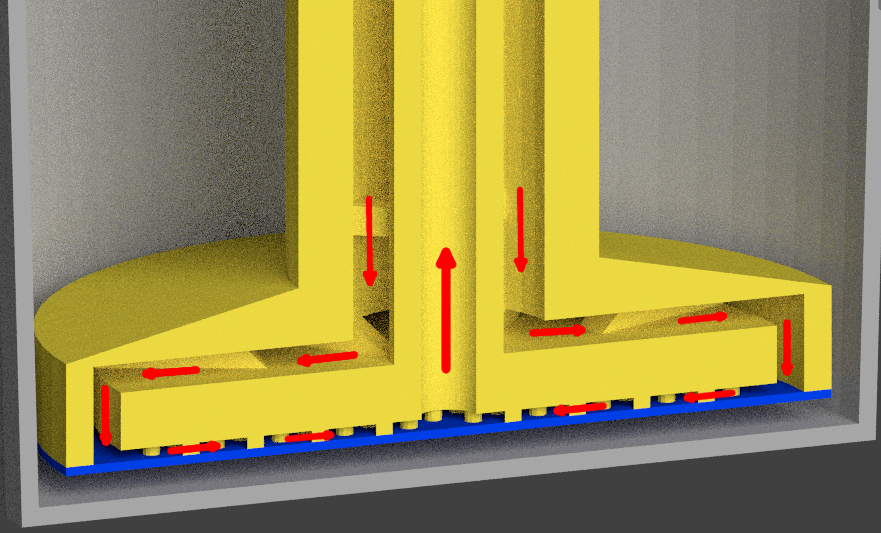
\includegraphics[scale=0.2]{../presentation-figures/piller-well-render-with-arrows.png} % remove for manuscript submission
\caption{
{\bf CAD rendering of the piller bottom.} The 'Pipe with in a pipe' flow pattern delivers gas to the bottom of each well where it diffuses to the culture.  
}
\label{piller-well-render-figure}
\end{figure}

\begin{figure}
%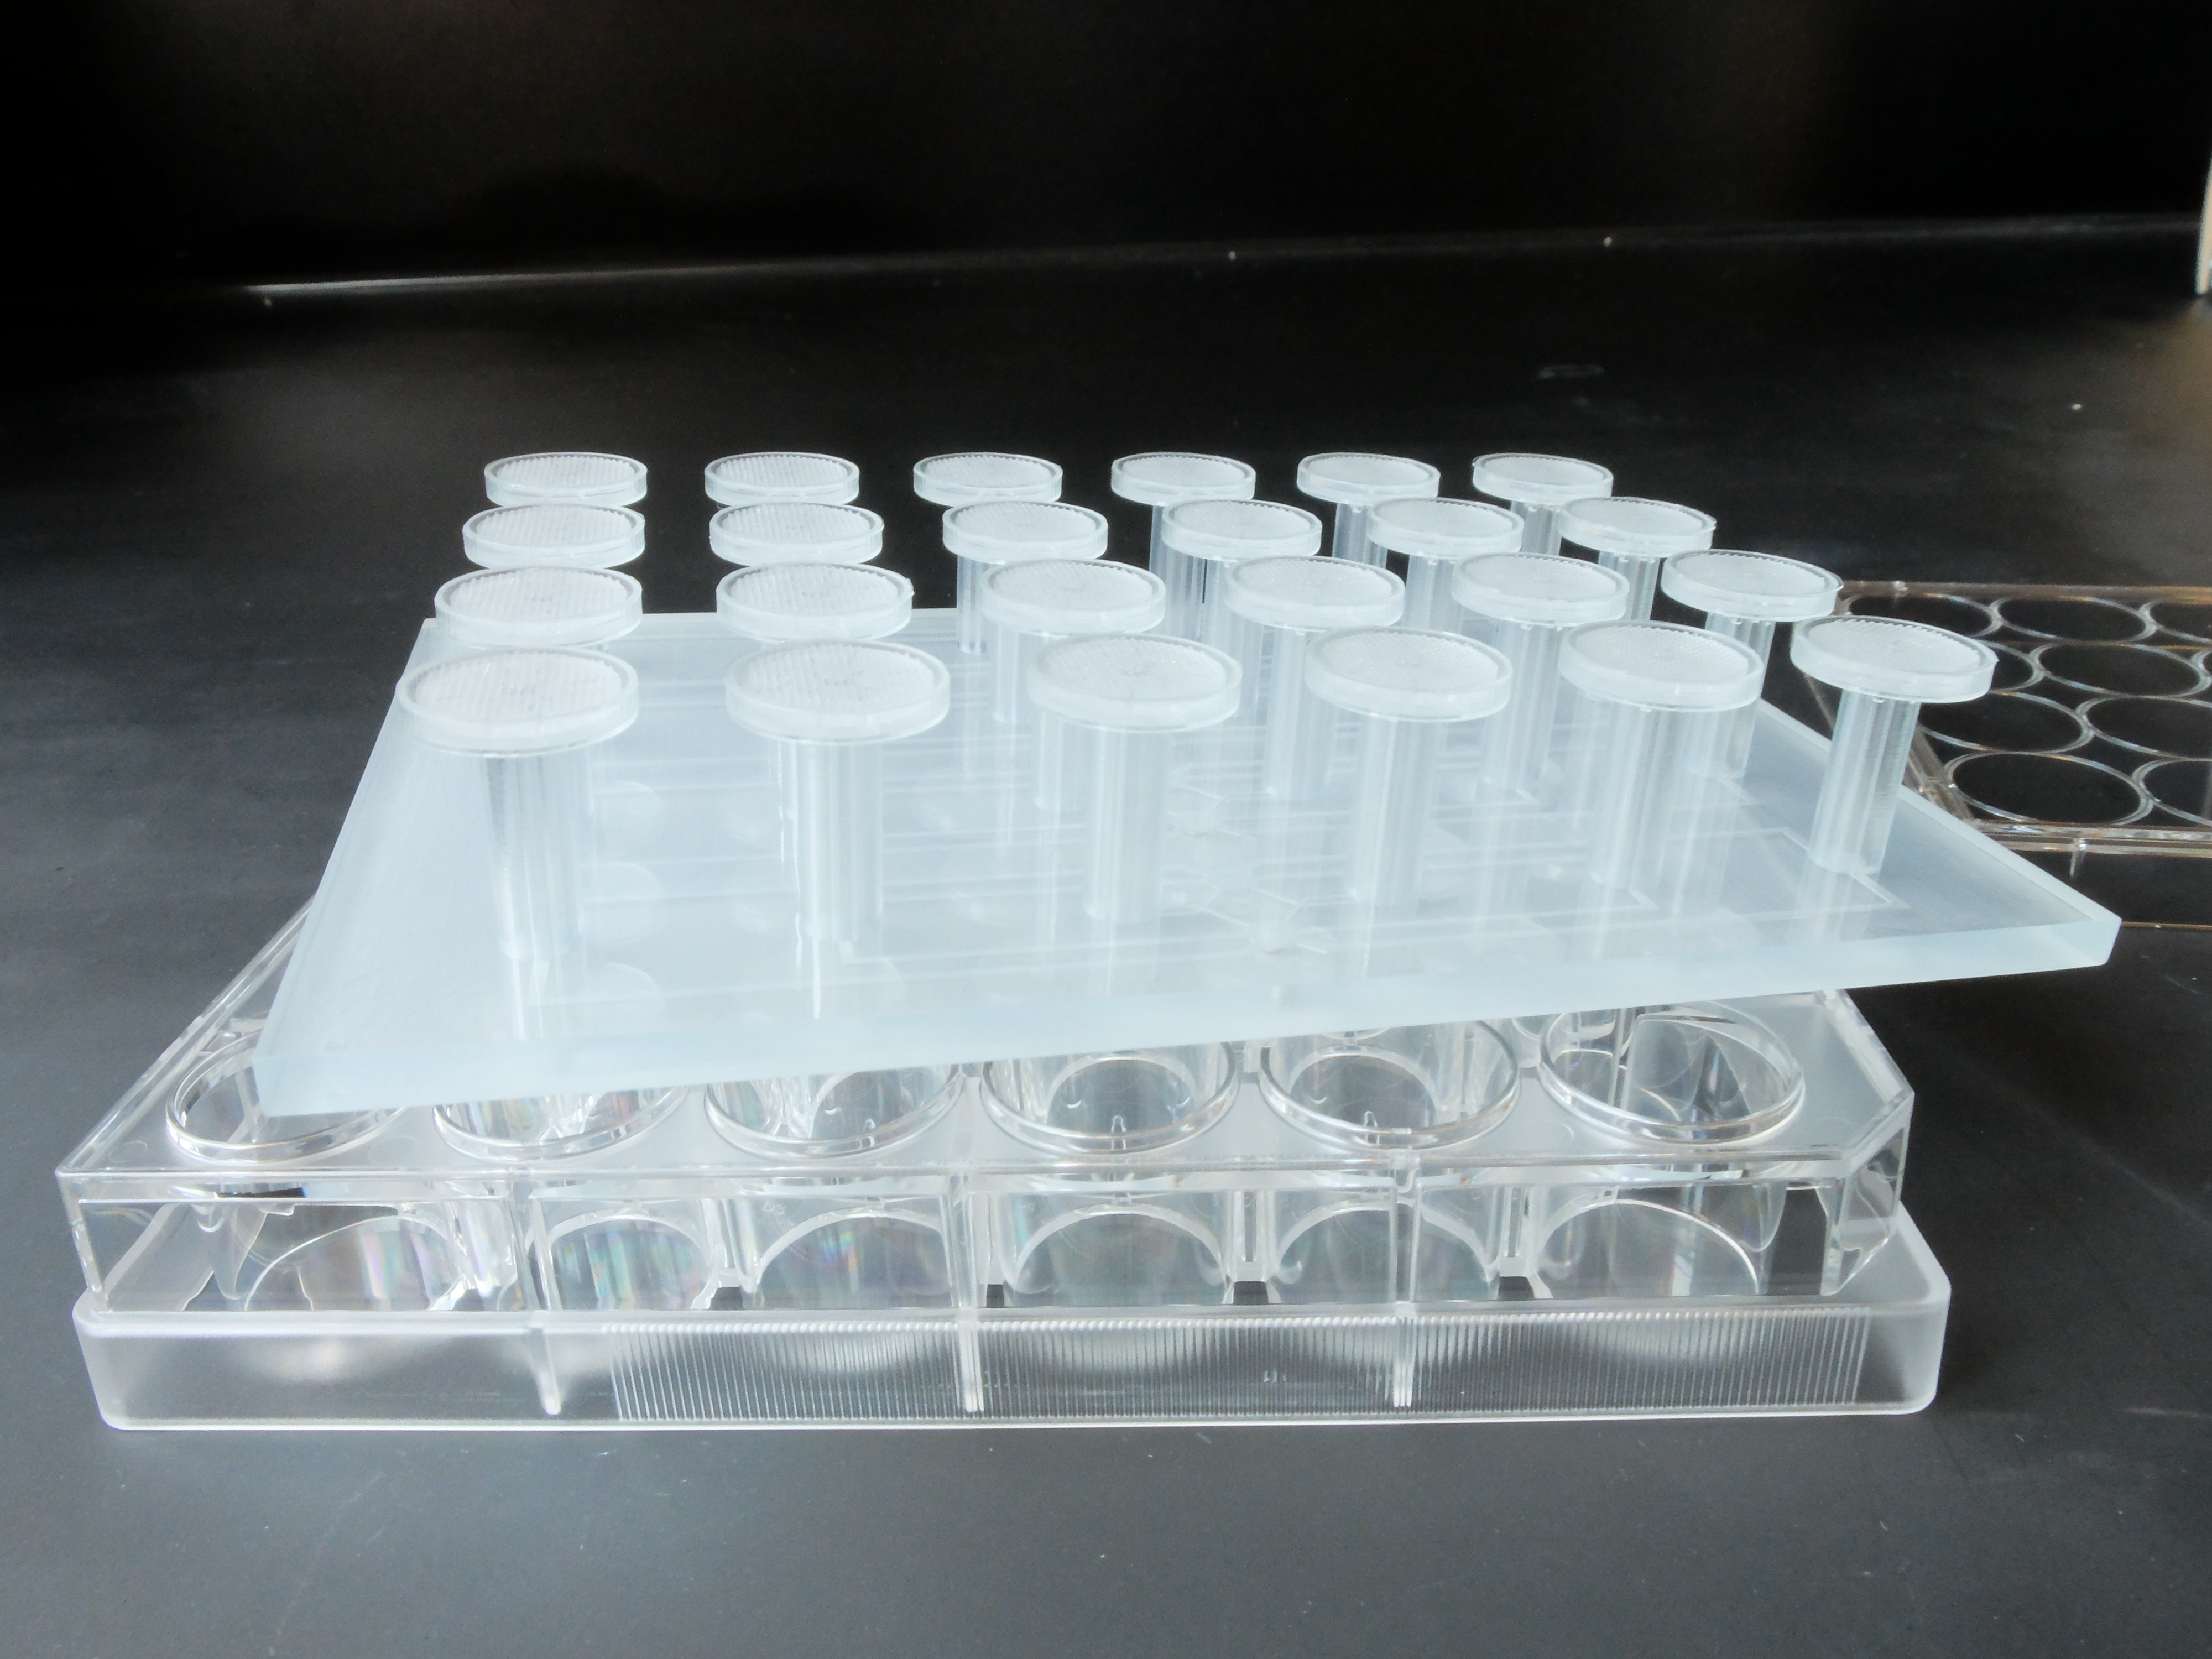
\includegraphics[scale=0.05]{../presentation-figures/24well.JPG} % remove for manuscript submission
%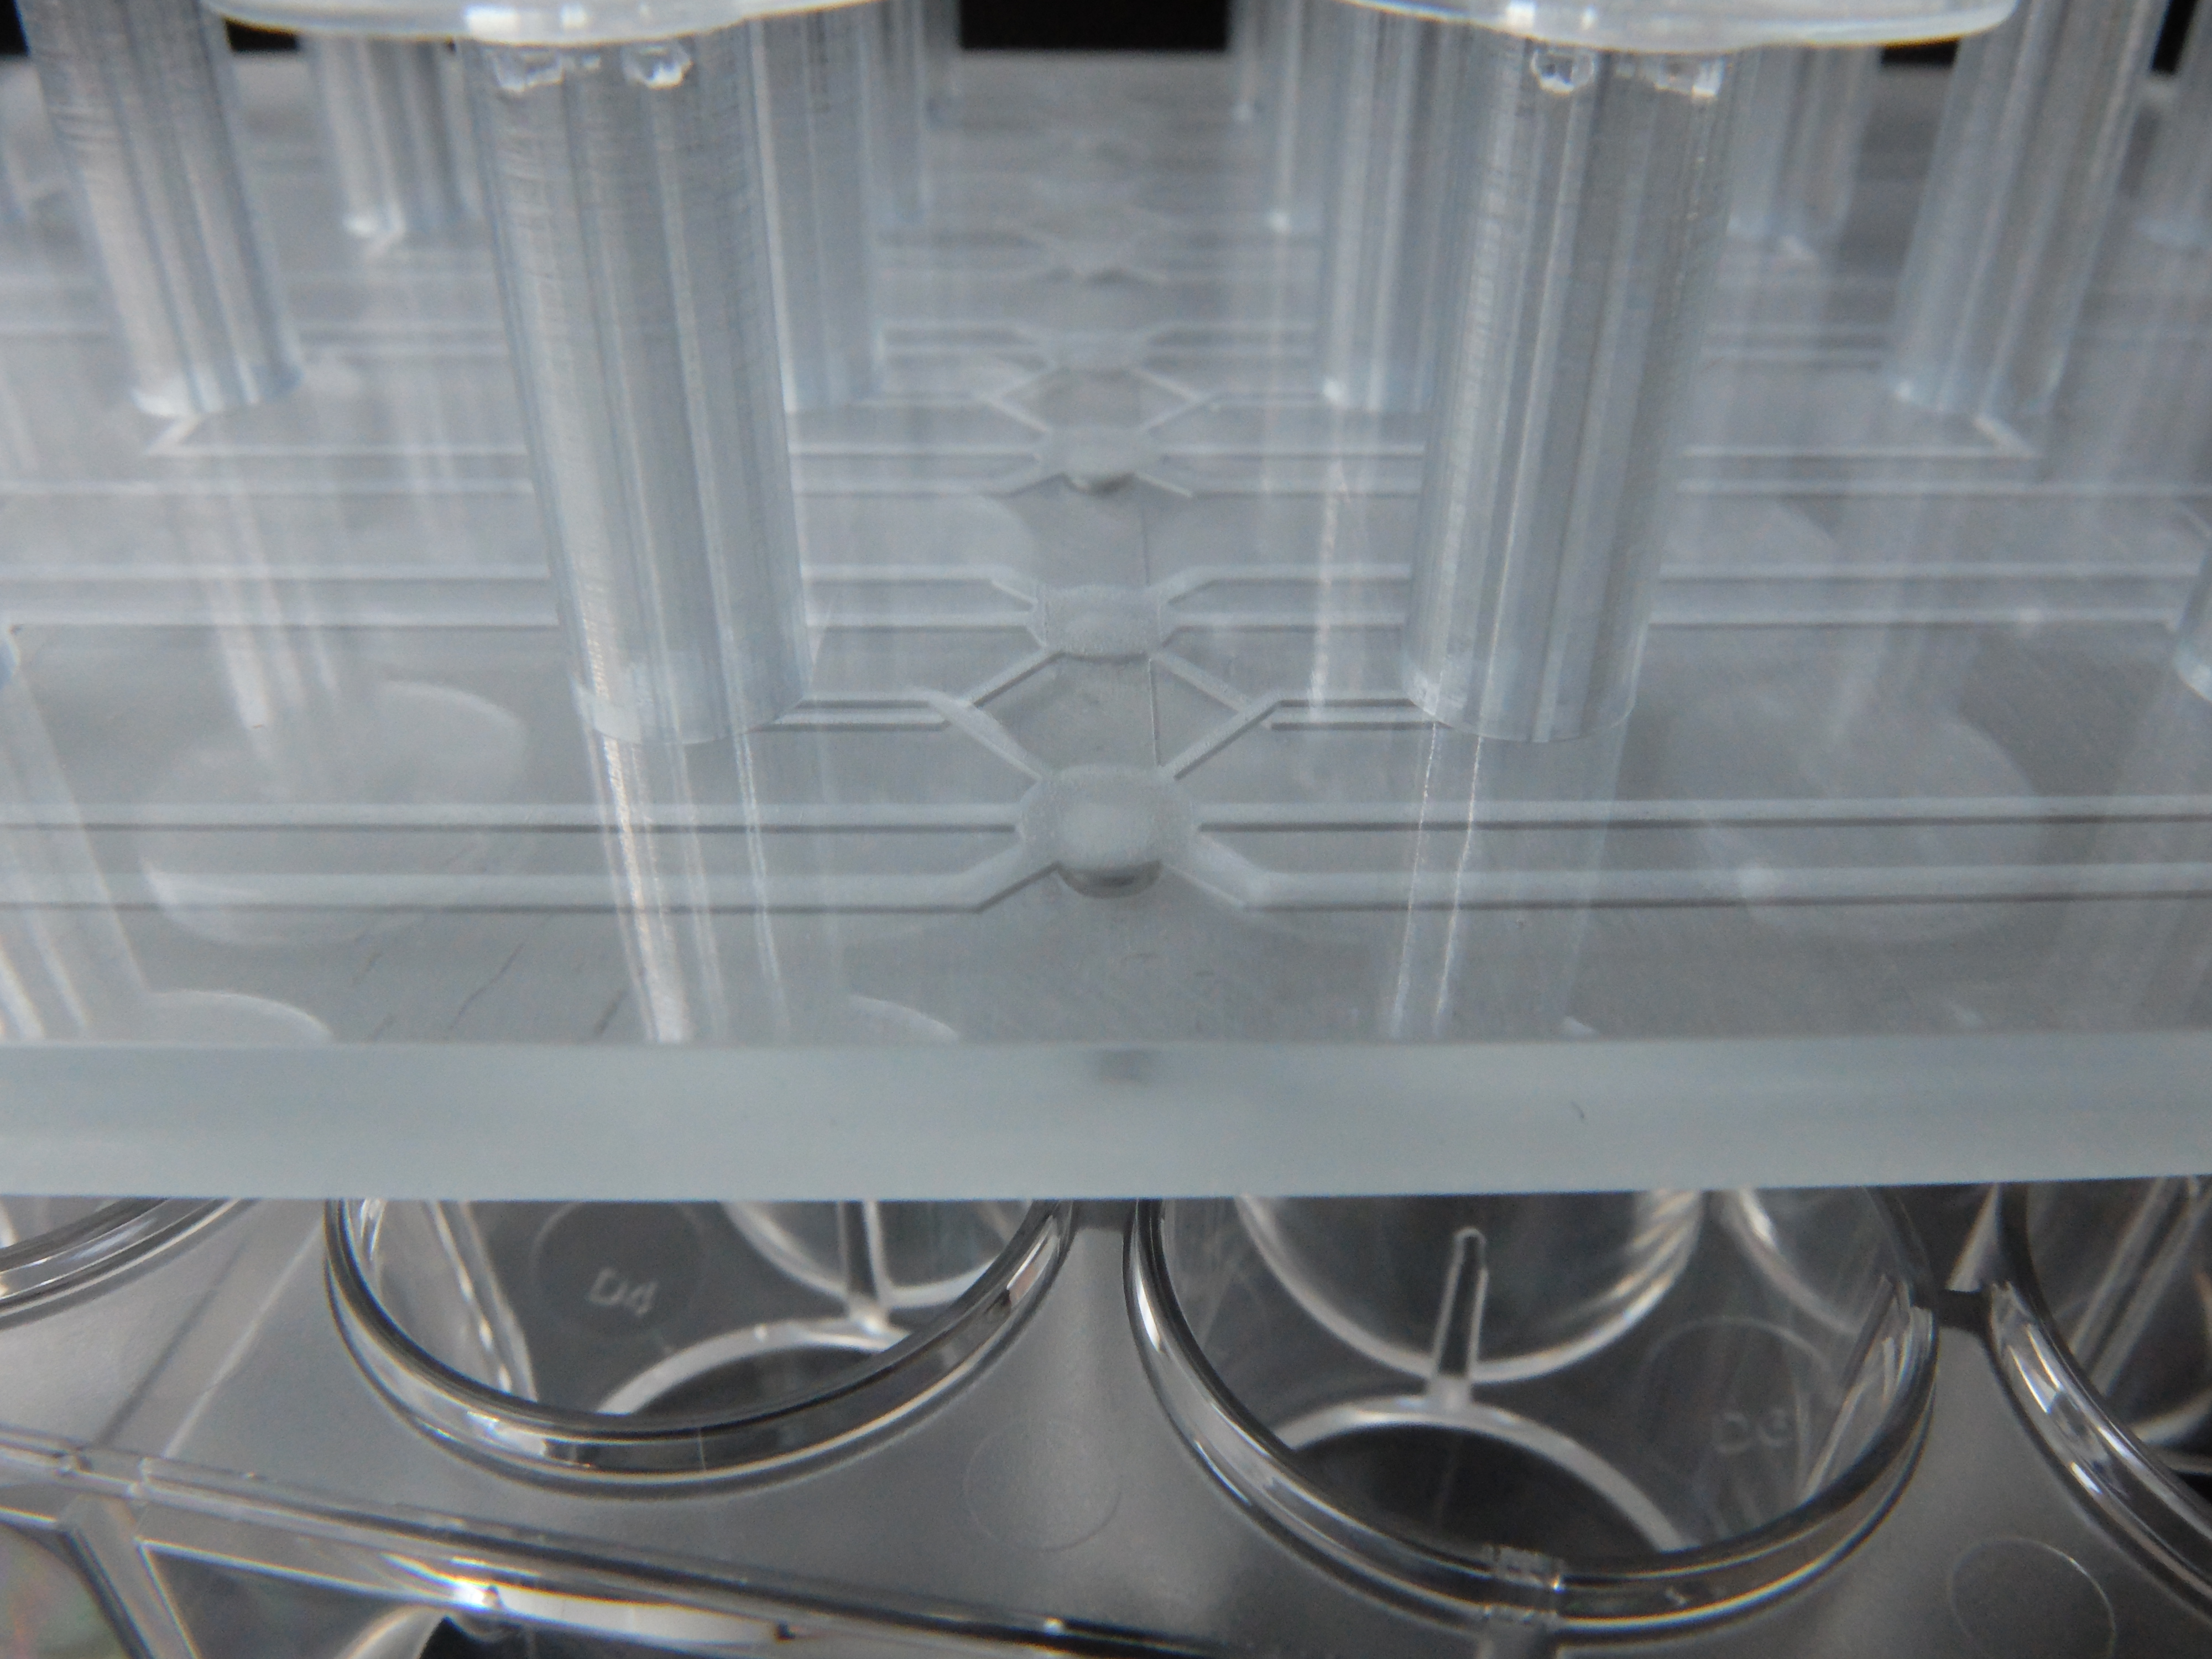
\includegraphics[scale=0.05]{../presentation-figures/printed-network.JPG} % remove for manuscript submission
\caption{
{\bf Photographs of the printed device.}  The printed device with membranes adhered. The distribution network is printed completely in resin.
}
\label{device-photos-figure}
\end{figure}

\begin{figure}
%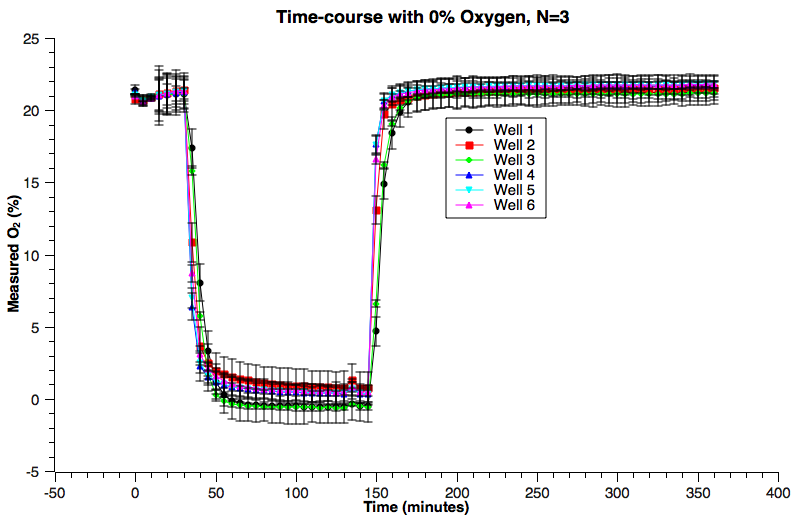
\includegraphics[scale=0.3]{../presentation-figures/6-well-plot.png} % remove for manuscript submission
%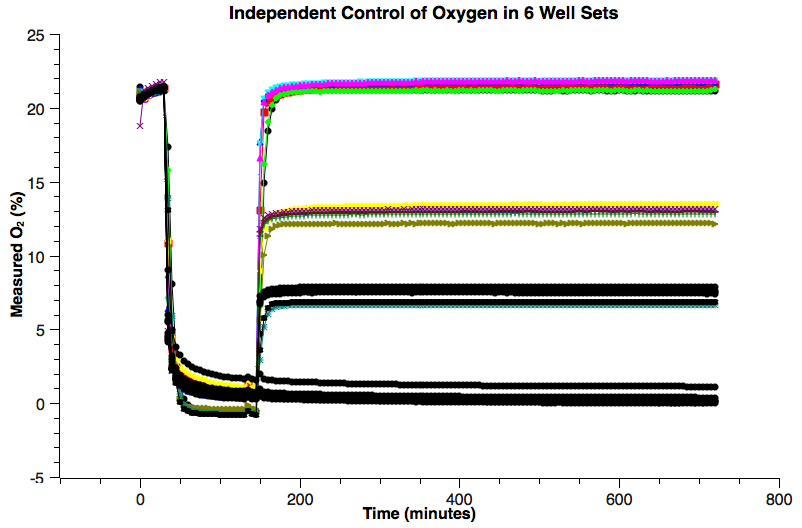
\includegraphics[scale=0.3]{../presentation-figures/24-well-plot.png} % remove for manuscript submission
\caption{
{\bf Oxygen Characterization.}  Time course data of oxygen being evacuated from the culture area as 0\% oxygen gas is perfused through the device. Each 6 well row of the plate can be controlled independently.  
}
\label{oxygen-char-figure}
\end{figure}

\begin{figure}
%\includegraphics[scale=0.2]{image.jpg} % remove for manuscript submission
\caption{
{\bf PCR Data.}  Not finished yet.  
}
\label{pcr-data}
\end{figure}



\section*{Tables}
% 
% See introductory notes if you wish to include sideways tables.
%
% NOTE: Please look over our table guidelines at http://www.plosone.org/static/figureGuidelines#tables to make sure that your tables meet our requirements. Certain types of spacing, cell merging, and other formatting tricks may have unintended results and will be returned for revision.
%
%\begin{table}[!ht]
%\caption{
%\bf{Table title}}
%\begin{tabular}{|c|c|c|}
%table information
%\end{tabular}
%\begin{flushleft}Table caption
%\end{flushleft}
%\label{tab:label}
% \end{table}

\section*{Supporting Information Legends}
%
% Please enter your Supporting Information captions below in the following format:
%\item{\bf Figure SX. Enter mandatory title here.} Enter optional descriptive information here.
% 
%\begin{description}
%\item {\bf}
%\item {\bf}
%\end{description}

\end{document}

